\documentclass[tikz,border=4pt]{standalone}
\usepackage{amsmath,amssymb,bm,setspace}
\usepackage{tikz,pgfplots}
\pgfplotsset{compat=1.18}
\usetikzlibrary{arrows.meta,calc,positioning,decorations.pathreplacing}
\begin{document}
% Schematic of the physical contact set-up, drawn from photographs of the rig.
% (a) side elevation of the arrangement, (b) the contact geometry it defines.
% Uses only tikz + arrows.meta/calc, which config/packages.tex already loads.
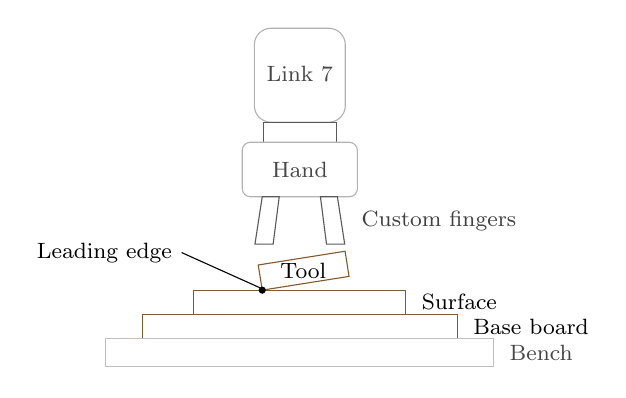
\begin{tikzpicture}[
    scale=0.77,
    font=\small,
    wood/.style={draw=brown!70!black, fill=white},
    woodDark/.style={draw=brown!70!black, fill=white},
    metal/.style={draw=gray!70!black, fill=white},
    robot/.style={draw=gray!60, fill=white},
    frameArrow/.style={-{Latex[length=2mm]}, thick},
  ]

% ============================ (a) side elevation =========================
\begin{scope}

  % ---- last robot link and flange -------------------------------------
  \draw[robot, rounded corners=6pt] (-0.75,5.75) rectangle (0.75,7.30);
  \node[gray!55!black] at (0,6.55) {\footnotesize Link 7};
  \draw[metal] (-0.60,5.42) rectangle (0.60,5.75);

  % ---- gripper body ---------------------------------------------------
  \draw[robot, rounded corners=3pt] (-0.95,4.52) rectangle (0.95,5.42);
  \node[gray!55!black] at (0,4.97) {\footnotesize Hand};

  % ---- custom aluminium fingers ---------------------------------------
  \draw[metal] (-0.62,4.52) -- (-0.74,3.74) -- (-0.44,3.74) -- (-0.34,4.52) -- cycle;
  \draw[metal] ( 0.62,4.52) -- ( 0.74,3.74) -- ( 0.44,3.74) -- ( 0.34,4.52) -- cycle;
  \node[gray!50!black, anchor=west] at (0.86,4.12) {\footnotesize Custom fingers};

  % ---- wooden tool -----------------------------------------------------
  % Anchored so its lower-left corner sits exactly on the surface: the
  % residual orientation error leaves the face a few degrees off parallel,
  % so one edge makes contact first.
  \begin{scope}[shift={(-0.62,2.98)}, rotate=9]
    \draw[woodDark] (0,0) rectangle (1.45,0.42);
    \node[font=\footnotesize] at (0.72,0.21) {Tool};
  \end{scope}

  % ---- contact surface and bench --------------------------------------
  \draw[wood] (-1.75,2.58) rectangle (1.75,2.98);        % raised strip
  \draw[wood] (-2.60,2.18) rectangle (2.60,2.58);        % base board
  \draw[fill=white, draw=gray!50] (-3.20,1.72) rectangle (3.20,2.18);
  \node[anchor=west] at (1.85,2.78) {\footnotesize Surface};
  \node[anchor=west] at (2.70,2.38) {\footnotesize Base board};
  \node[gray!55!black, anchor=west] at (3.30,1.95) {\footnotesize Bench};

  % ---- contact marker ---------------------------------------------------
  \fill[black] (-0.62,2.98) circle (1.7pt);
  \draw[black, thin] (-0.66,3.02) -- (-1.95,3.60);
  \node[black, anchor=east, font=\footnotesize] at (-1.95,3.60)
        {Leading edge};

  
\end{scope}


\end{tikzpicture}

\end{document}
